\documentclass[aspectratio=169, 10pt]{beamer}

%--- Packages ---
\usepackage[utf8]{inputenc}
\usepackage{tikz}
\usepackage{pgfplots}
\usepackage{booktabs}
\usepackage{amsmath}
\usetikzlibrary{calc, intersections}

%--- Theme Settings ---
\usetheme{Madrid}
\usecolortheme{beaver} % Red/Grey theme often good for Econ
\setbeamerfont{title}{series=\bfseries,parent=structure}
\setbeamerfont{frametitle}{series=\bfseries,parent=structure}

% Title Information
\title{Unit 4: Perfect Competition}
\subtitle{Characteristics, Profit Maximization, and Efficiency}
\author{Doğukan Günkördü}
\date{}

\begin{document}

%--- Title Slide ---
\begin{frame}
    \titlepage
\end{frame}

%--- Agenda ---
\begin{frame}{Learning Objectives}
    \begin{itemize}
        \item Understand the characteristics of Perfect Competition.
        \item Analyze the relationship between Market Demand and Firm Demand.
        \item Calculate Profit Maximization ($MR = MC$).
        \item Apply the Shut-Down Rule in the short run.
        \item Analyze Long-Run equilibrium and adjustments.
        \item Define Allocative and Productive Efficiency.
    \end{itemize}
\end{frame}

%===========================================================
% SECTION 1: CHARACTERISTICS & DEMAND
%===========================================================
\section{Characteristics \& Demand}

\begin{frame}{Market Structures Overview}
    The "Market Structure" is defined by the level of competition.
    \vspace{0.5cm}
    
    \begin{center}
    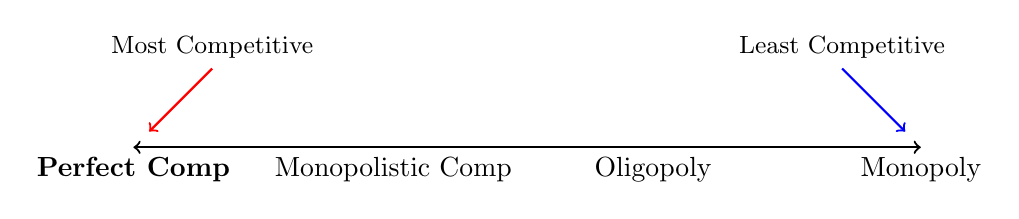
\begin{tikzpicture}
        \draw[<->, thick] (0,0) -- (10,0);
        \node[below] at (0,0) {\textbf{Perfect Comp}};
        \node[below] at (3.3,0) {Monopolistic Comp};
        \node[below] at (6.6,0) {Oligopoly};
        \node[below] at (10,0) {Monopoly};
        
        \draw[->, thick, red] (1, 1) -- (0.2, 0.2);
        \node[above] at (1,1) {\small Most Competitive};
        
        \draw[->, thick, blue] (9, 1) -- (9.8, 0.2);
        \node[above] at (9,1) {\small Least Competitive};
    \end{tikzpicture}
    \end{center}
    
    \begin{block}{Why it matters}
    Different firms face vastly different levels of competition. A lettuce farmer has less pricing power than a cable company.
    \end{block}
\end{frame}

\begin{frame}{Characteristics of Perfect Competition}
    \begin{enumerate}
        \item \textbf{Many Small Firms:} Large number of sellers competing in national/global markets.
        \item \textbf{Identical Products:} Goods are perfect substitutes (e.g., corn, strawberries).
        \item \textbf{Easy Entry and Exit:} No significant barriers to start or stop producing.
        \item \textbf{Price Takers:} Firms have \textit{no influence} on price. They must sell at the market equilibrium price.
    \end{enumerate}
\end{frame}

\begin{frame}{The "Price Taker" Concept}
    Because the firm sells an identical product in a massive market:
    \begin{itemize}
        \item If they charge \textbf{above} market price: Consumers buy elsewhere (sales = 0).
        \item If they charge \textbf{below} market price: They lose revenue unnecessarily.
    \end{itemize}
    \vspace{0.3cm}
    \textbf{Result:} The Firm's Demand Curve is \textbf{Perfectly Elastic} (Horizontal).
\end{frame}

\begin{frame}{Market vs. Firm Graph (Side-by-Side)}
    \begin{columns}
        \column{0.5\textwidth}
        \centering
        \textbf{The Market}
        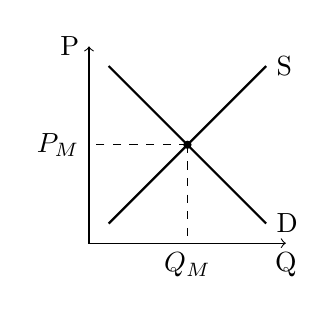
\begin{tikzpicture}[scale=0.5]
            \draw[<->] (0,5) node[left]{P} -- (0,0) -- (5,0) node[below]{Q};
            \draw[thick] (0.5,4.5) -- (4.5,0.5) node[right]{D};
            \draw[thick] (0.5,0.5) -- (4.5,4.5) node[right]{S};
            \draw[dashed] (2.5,2.5) -- (0,2.5) node[left]{$P_M$};
            \draw[dashed] (2.5,2.5) -- (2.5,0) node[below]{$Q_M$};
            \fill (2.5,2.5) circle (3pt);
        \end{tikzpicture}
        
        \column{0.5\textwidth}
        \centering
        \textbf{The Firm}
        \begin{tikzpicture}[scale=0.5]
            \draw[<->] (0,5) node[left]{P} -- (0,0) -- (5,0) node[below]{Q};
            % Horizontal Demand
            \draw[thick, blue] (0,2.5) -- (4.8,2.5) node[right]{$P=MR=D=AR$};
            \draw[dashed] (-2.5,2.5) -- (0,2.5); % Connection line
        \end{tikzpicture}
    \end{columns}
    
    \vspace{0.5cm}
    \begin{alertblock}{Exam Tip: Mr. DARP}
    For a perfectly competitive firm:
    \[ \textbf{M}arginal \textbf{R}evenue = \textbf{D}emand = \textbf{A}verage \textbf{R}evenue = \textbf{P}rice \]
    \end{alertblock}
\end{frame}

%===========================================================
% SECTION 2: PROFIT MAXIMIZATION
%===========================================================
\section{Profit Maximization}

\begin{frame}{Profit Maximizing Rule}
    \begin{block}{The Golden Rule}
    All firms maximize profit (or minimize loss) by producing where:
    \[ \textbf{MR} = \textbf{MC} \]
    \end{block}
    
    \begin{itemize}
        \item \textbf{If MR > MC:} Produce more. Revenue from the next unit exceeds the cost to make it.
        \item \textbf{If MC > MR:} Produce less. The cost to make the last unit was higher than the revenue it brought in.
        \item \textbf{Economic Profit Formula:} $(P - ATC) \times Q$
    \end{itemize}
\end{frame}

\begin{frame}{Short-Run Economic Profit}
    \begin{columns}
        \column{0.4\textwidth}
        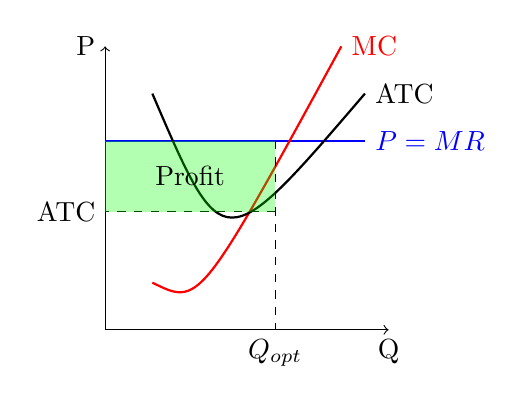
\begin{tikzpicture}[scale=0.6]
            \draw[<->] (0,6) node[left]{P} -- (0,0) -- (6,0) node[below]{Q};
            
            % MR = P
            \draw[thick, blue] (0,4) -- (5.5,4) node[right]{$P=MR$};
            
            % MC Curve (checkmark shape)
            \draw[thick, red] (1,1) .. controls (2,0.5) .. (5,6) node[right]{MC};
            
            % ATC Curve (U shape, min below P)
            \draw[thick] (1,5) .. controls (2.5,1.5) .. (5.5,5) node[right]{ATC};
            
            % Intersection MR=MC
            \draw[dashed] (3.6,4) -- (3.6,0) node[below]{$Q_{opt}$};
            
            % ATC at Qopt
            \draw[dashed] (3.6,2.5) -- (0,2.5) node[left]{ATC};
            
            % Profit Box
            \fill[green, opacity=0.3] (0,2.5) rectangle (3.6,4);
            \node at (1.8, 3.25) {Profit};
        \end{tikzpicture}
        
        \column{0.6\textwidth}
        \textbf{Steps to graph:}
        \begin{enumerate}
            \item Find where $MR = MC$. This determines quantity ($Q_{opt}$).
            \item Go down from $Q_{opt}$ to the ATC curve.
            \item The rectangular area between Price and ATC is the profit.
        \end{enumerate}
        \vspace{0.2cm}
        \textit{Note: If $P > ATC$, the firm earns Economic Profit.}
    \end{columns}
\end{frame}

%===========================================================
% SECTION 3: THE SHUT-DOWN RULE
%===========================================================
\section{The Shut-Down Rule}

\begin{frame}{Losses and The Shut-Down Rule}
    What if Price falls below ATC? The firm makes a loss.
    
    \begin{itemize}
        \item \textbf{Option 1 (P > AVC):} \textit{Keep Producing.} 
        \begin{itemize}
            \item The firm covers all variable costs and \textit{some} fixed costs.
            \item Losses are smaller than if they shut down (where loss = Total Fixed Cost).
        \end{itemize}
        
        \item \textbf{Option 2 (P < AVC):} \textit{Shut Down.}
        \begin{itemize}
            \item The price doesn't even cover the variable inputs (labor, materials).
            \item Every unit produced \textit{adds} to losses.
            \item Firm shuts down and just pays Fixed Costs.
        \end{itemize}
    \end{itemize}
\end{frame}

\begin{frame}{The Shut-Down Graph}
    \begin{center}
    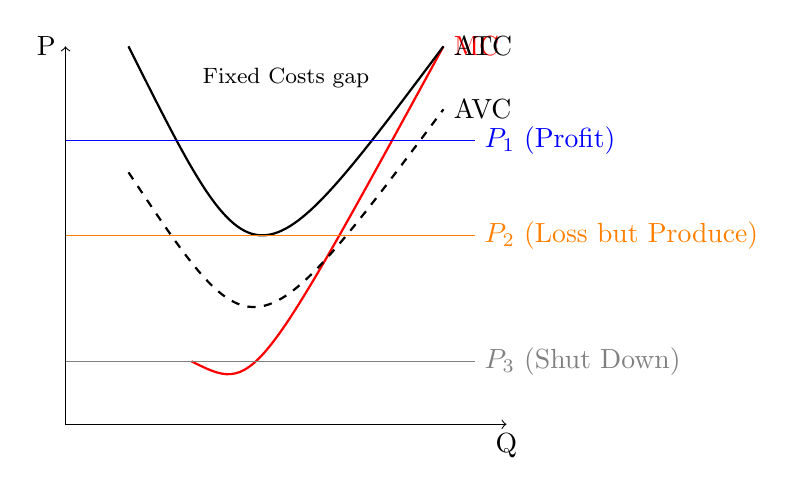
\begin{tikzpicture}[scale=0.8]
        \draw[<->] (0,6) node[left]{P} -- (0,0) -- (7,0) node[below]{Q};
        
        % Curves
        \draw[thick, red] (2,1) .. controls (3,0.5) .. (6,6) node[right]{MC};
        \draw[thick] (1,6) .. controls (3,2) .. (6,6) node[right]{ATC};
        \draw[thick, dashed] (1,4) .. controls (3,1) .. (6,5) node[right]{AVC};
        
        % Prices
        \draw[blue] (0, 4.5) -- (6.5,4.5) node[right]{$P_1$ (Profit)};
        \draw[orange] (0, 3) -- (6.5,3) node[right]{$P_2$ (Loss but Produce)};
        \draw[gray] (0, 1) -- (6.5,1) node[right]{$P_3$ (Shut Down)};
        
        \node[font=\footnotesize] at (3.5, 5.5) {Fixed Costs gap};
    \end{tikzpicture}
    \end{center}
    \textbf{Rule:} The firm's supply curve is the MC curve \textbf{above} the AVC.
\end{frame}

%===========================================================
% SECTION 4: LONG RUN & EFFICIENCY
%===========================================================
\section{Long Run \& Efficiency}

\begin{frame}{Long-Run Adjustment}
    In the long run, firms can enter and exit the market.
    
    \begin{columns}
        \column{0.5\textwidth}
        \begin{block}{Scenario 1: Economic Profits}
            \begin{enumerate}
                \item Firms earn profits ($P > ATC$).
                \item New firms \textbf{ENTER} the market.
                \item Market Supply shifts \textbf{RIGHT}.
                \item Market Price \textbf{FALLS}.
                \item Profits disappear ($P = ATC$).
            \end{enumerate}
        \end{block}
        
        \column{0.5\textwidth}
        \begin{block}{Scenario 2: Economic Losses}
            \begin{enumerate}
                \item Firms incur losses ($P < ATC$).
                \item Firms \textbf{EXIT} the market.
                \item Market Supply shifts \textbf{LEFT}.
                \item Market Price \textbf{RISES}.
                \item Losses disappear ($P = ATC$).
            \end{enumerate}
        \end{block}
    \end{columns}
\end{frame}

\begin{frame}{Long-Run Equilibrium Graph}
    In the Long Run, the firm breaks even (Zero Economic Profit / Normal Profit).
    
    \begin{center}
    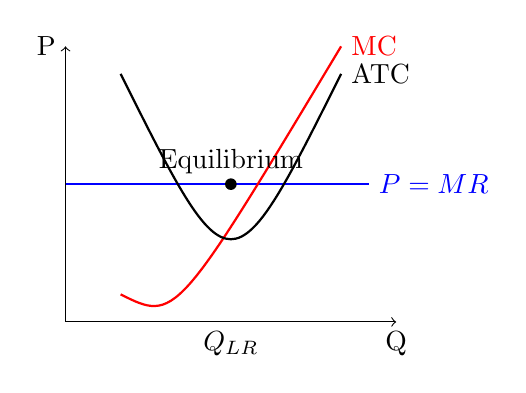
\begin{tikzpicture}[scale=0.7]
        \draw[<->] (0,5) node[left]{P} -- (0,0) -- (6,0) node[below]{Q};
        
        % P = MR
        \draw[thick, blue] (0,2.5) -- (5.5,2.5) node[right]{$P = MR$};
        
        % MC
        \draw[thick, red] (1,0.5) .. controls (2,0) .. (5,5) node[right]{MC};
        
        % ATC Tangent to P
        \draw[thick] (1,4.5) .. controls (3,0.5) .. (5,4.5) node[right]{ATC};
        
        \fill (3,2.5) circle (3pt);
        \node[above] at (3,2.5) {Equilibrium};
        \node[below] at (3,0) {$Q_{LR}$};
        
    \end{tikzpicture}
    \end{center}
    At this point: $P = MC = \text{Minimum ATC}$.
\end{frame}

\begin{frame}{Types of Efficiency}
    Perfect Competition is unique because it achieves \textbf{both} types of efficiency in the long run.
    \vspace{0.5cm}
    
    \begin{block}{1. Allocative Efficiency ($P = MC$)}
        \begin{itemize}
            \item Firms produce the exact amount society desires.
            \item Price (social benefit) equals Marginal Cost (social cost).
            \item No Deadweight Loss.
        \end{itemize}
    \end{block}

    \begin{block}{2. Productive Efficiency ($P = \text{Minimum } ATC$)}
        \begin{itemize}
            \item Goods are produced at the lowest possible cost.
            \item Using the fewest possible resources.
            \item Forces firms to use the best available technology.
        \end{itemize}
    \end{block}
\end{frame}

%===========================================================
% SECTION 5: SUMMARY & PRACTICE
%===========================================================
\section{Summary}

\begin{frame}{Summary Checklist}
    \begin{itemize}
        \item \textbf{Graphs:} Can you draw Market and Firm side-by-side?
        \item \textbf{Labels:} Remember $MR = D = AR = P$ (Mr. Darp).
        \item \textbf{Calculations:} 
            \begin{itemize}
                \item Profit = $(P - ATC) \times Q$
                \item Total Cost = $ATC \times Q$
                \item TFC = $(ATC - AVC) \times Q$
            \end{itemize}
        \item \textbf{Decisions:}
            \begin{itemize}
                \item $MR = MC$: How much to produce.
                \item $P < AVC$: When to shut down.
            \end{itemize}
        \item \textbf{Long Run:} Entry/Exit drives profits to zero.
    \end{itemize}
\end{frame}

\end{document}
